\chapter{Design}
\label{Chapter:Design}

This chapter discusses the design considerations taken during the design development of the system. The design stage is very important since it lays down the foundation for the whole system.
Thus a considerable amount of time has been spent in designing the system. \citet[12]{bell2005} states that about 5\% of the total time that takes for the development of a software should be spent for the design state alone. For comparison, the coding process takes about 7\%; Testing takes 8\%. 

The design process has gone through many iterations to ensure the best possible quality of the product. The research presented in chapter \ref{Chapter:Literature-Review} has affected immensely the design, especially section \ref{section:commercial-har-systems}. The design can be split into four main sections, namely Mobile Platform and IDE; Database Design; Architectural design and User Interface (UI).

    \section{Mobile Platform and IDE}
        The first point that was considered in the design process was the \textbf{mobile platform} on which the proposed application will be implemented and distributed. After research on the current market, Google's \textit{Android} was fount to dominate in Europe \citep{williams2016}. Android-based smartphones hold 75.6\% of market share dominating other mobile platforms such as Apple's \textit{iOS} and Microsoft's \textit{Windows Phone}. Thus, Android OS was chosen to form the basis of the proposed mobile application since it will allow the application to be downloaded and used by as many people as possible.
        
        After choosing the mobile platform, one important decision is to choose the development environment or the \textbf{Integrated Development Environment} (\gls{ide}) that will be used to develop the application. That was an easy decision since Android Studio is known to be the official \gls{ide} for Android development \citep{androidstudio2017}.

    \section{Database Design}
    This section discuses the design of the database system that will be used to store data of \textit{"Active Minutes"} mobile application. The design of the database can be seen in figure \ref{fig:data_modeling_er_diagram}. It includes the following entities \textbf{User}, \textbf{Activity} and \textbf{Training\_data}. The following sections will explain the responsibilities of each entity (i.e.\ database tables).
        
        \subsection{Entity Relationship Model}
        
        \begin{figure}[ht]
            \centering
            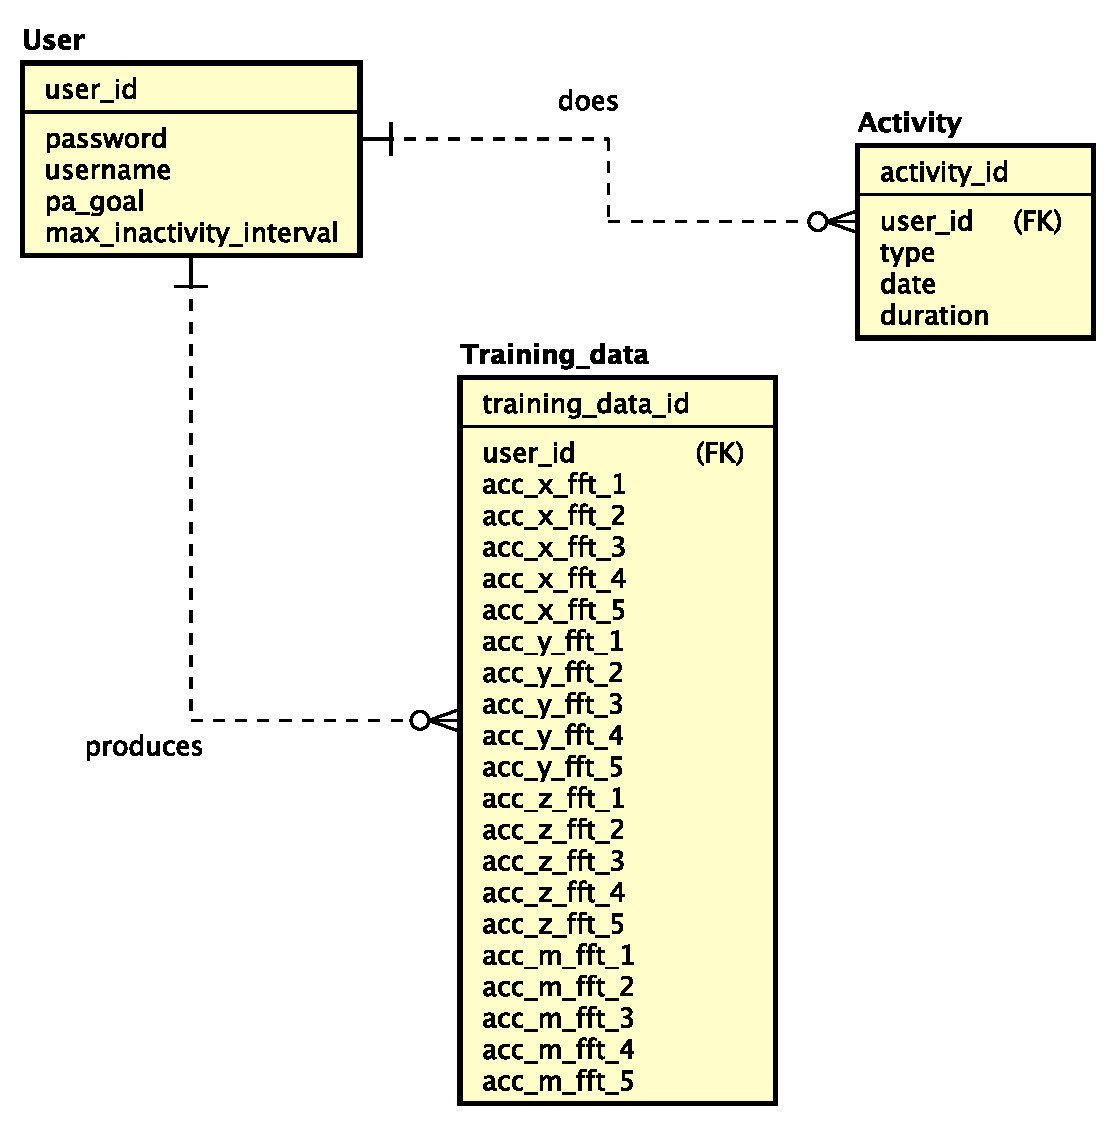
\includegraphics[width=12cm]{data_modeling_er_diagram}
            \caption{Database ER Diagram}
            \label{fig:data_modeling_er_diagram}
        \end{figure}
        
        \subsubsection{Entities}
        
        \begin{itemize}
            \item User(user\_id, password, username, pa\_goal,max\_inactivity\_time)
            \item Training\_data(user\_id, acc\_x\_fft\_1, acc\_x\_fft\_2, acc\_x\_fft\_3, acc\_x\_fft\_4...)
            \item Activity(activity\_id, user\_id, type, date, duration)
        \end{itemize}
        
        \subsubsection{Relationships}
        \begin{itemize}
        \item Does --- User does Activity [1:m][m:o]
        \item Produces --- User produces Training\_data [1:m][m:o]
        \end{itemize}
        
        \subsubsection{User}
        The user table is responsible for storing the personal information of every registered user. For example, \textit{user\_id} (number) will allow every user to be uniquely identified so further information can be accessed. The table will also store the \textit{username} and \textit{password} of every user. These fields are used for the authenticating different users of the application upon login.
        
        Also, the user table will store additional information such as the \gls{pa} goal and the maximum sedentary time (both in minutes) before a notification is send to remind the current logged-in user for the prolonged inactivity.   
        
        \subsubsection{Activity}
        
        \subsubsection{Training\_data}
    
    
    \section{Architectural design}
    This section discuses the design of the system on a software level.
    
        
    \section{User Interface Design}
    TO BE DONE